\section{实验材料及方法}
本文是将商用AZ31B镁合金板材和1060纯铝板材制成铝-镁-铝夹层,进行不同道次及道次压下率复合轧制实验,并对轧制所得板材进行显微组织观察及力学性能分析研究。本章介绍了实验所采用的材料、样品制备方式及实验方法。\par
\subsection{实验流程图}
实验流程图\ref{fig:liuchengtu}。
\begin{figure}[H]
	\centering
	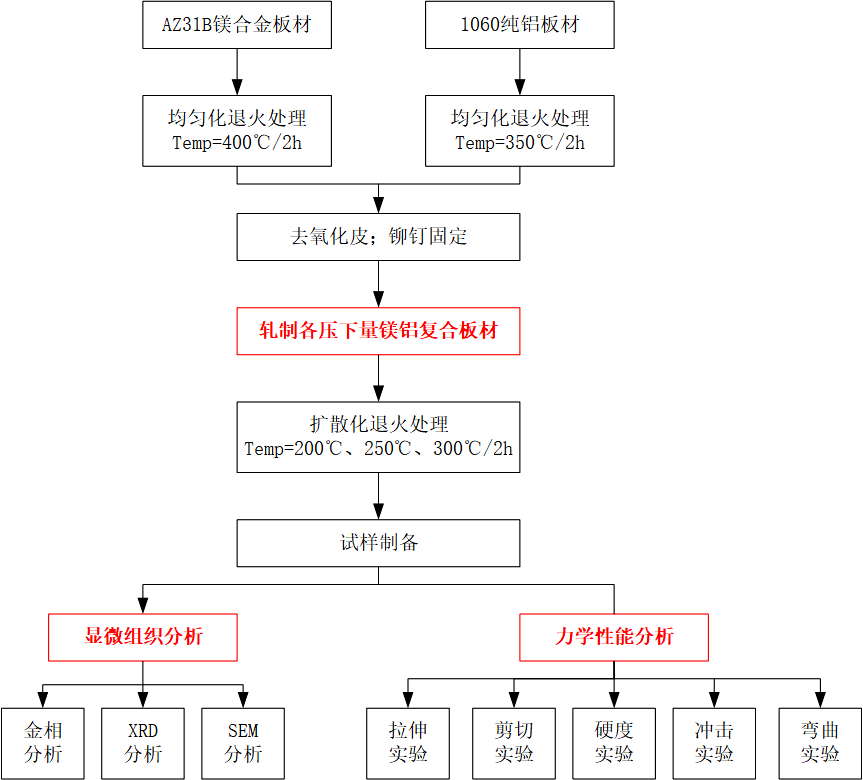
\includegraphics[width=0.5\textwidth]{images/liuchengtu.png}
	\caption{实验流程图}
	\label{fig:liuchengtu}
\end{figure}
\subsection{实验材料}
实验所采用的原始材料为商用AZ31B镁合金铸轧板材和1060铝板材。合金原材料采用连续铸轧工艺生产,生产工序经过配料/熔炼/静置/放料/连续铸轧等流程,由于原材料板材较大,采用剪板机进行切割取样。\par
公式格式:
\begin{equation}
\label{equ:maxwell}
    \begin{cases}
    \nabla\times\vec{E}=-\frac{\partial\vec{B}}{\partial t}\\
    \nabla\times\vec{H}=\vec{J_v}+\frac{\partial\vec{D}}{\partial t}\\
    \nabla\cdot\vec{D}=\rho_v\\
    \nabla\cdot\vec{B}=0
    \end{cases}\quad
    \begin{cases}
    \vec{D}=\epsilon\vec{E}\\
    \vec{B}=\mu\vec{H}\\
    \vec{J_v}=\sigma\vec{E}
    \end{cases}  
\end{equation}

表格格式:
\begin{table}[H]
    \centering
    \caption{一个表格}
    \zihao{5}
    \label{tab:all_parameters}
    \begin{tabular}{c c c l}
    \toprule[1.5pt]
    参数          & 数值         & 单位   & 备注     \\ 
    \midrule[0.5pt]
    $A$         & 2132   & 1      & A参数 \\
    $B$         & 3423   & 1      & B参数 \\ 
    $C$         & 1232   & 1      & C参数 \\ 
    $D$         & 1234   & μm     & D参数 \\
    $\alpha$    & 11.1   & cm     & α参数 \\
    $\beta$     & 123.3  & km     & β参数 \\       
    \bottomrule[1.5pt]
    \end{tabular}
\end{table}

\clearpage